% !TeX root = ../main.tex
% Add the above to each chapter to make compiling the PDF easier in some editors.

\chapter{Hidden Markov Models}\label{chapter:hmm}

One of the approaches to generate time series in this thesis are Hidden Markov Models (HMM). HMMs are a powerful tool to model observed data samples of a discrete time-series. They are a generative model which makes them inherently suitable for the task of generating data. It is a flexible approach: the observed data of the time series can be continuously or discretely distributed and the samples can be scalars or vectors. 

The theory of Hidden Markov Models was originally developed by Baum \parencite{baum1972inequality}. HMMs have a variety of applications. They are especially useful in speech and language related-tasks. They have been used in applications such as speech recognition, speech tagging, and machine translation\parencite{huang2001spoken}.

\section{Markov Chain}
To understand Hidden Markov models we first have to understand the regular \emph{Markov Chain}. Let $\mathbf{X}=X_{1}, X_{2}, \ldots X_{n}$ be a sequence of random variables. The probability of the sequence is $P\left(X_{1}, X_{2}, \ldots, X_{n}\right)$ and using Bayes rule get: 

\begin{equation}
P\left(X_{1}, X_{2}, \ldots, X_{n}\right)=P\left(X_{1}\right) \prod_{i=2}^{n} P\left(X_{i} |X_{1}, X_{2}, \ldots, X_{i-1}\right)
\end{equation}

This shows that the probability of variable $X_1$ is dependent on only itself. $X_2$ is conditioned on $X_1$, $X_3$ is conditioned on $X_1$ and $X_2$ and so on. To be a Markov Chain a sequence has to satisfy the Markov property, which states that the probability of a variable can only depend on its predecessor. Formally this means: 

\begin{equation}
P\left(X_{i} | X_{1}, X_{2}, \ldots, X_{i-1}\right)=P\left(X_{i} | X_{i-1}\right)
\end{equation}

And turns the previous equation to :

\begin{equation}
P\left(X_{1}, X_{2}, \ldots, X_{n}\right)=P\left(X_{1}\right) \prod_{i=2}^{n} P\left(X_{i} | X_{i-1}\right)
\end{equation}

A Markov Chain can be represented as a finite state machine. Each random variable $X_i$ corresponds to a state $s$ in the Markov chain. Every state transition has a probability $P(s | s')$ and because of the Markov property a state only depends on its predecessor state. With this representation a Markov Chain can be parametrized like this:

\begin{equation}
\begin{aligned}
&a_{i j}=P\left(s_{t}=j | s_{t-1}=i\right) \quad 1 \leq i, j \leq N \\
&\pi_{i}=P\left(s_{1}=i\right) \quad 1 \leq i \leq N \\
&\sum_{j=1}^{N} a_{i j}=1 ; \quad 1 \leq i \leq N \\
&\sum_{j=1}^{N} \pi_{j}=1
\end{aligned}
\end{equation}

Here $a_{ij}$ is the probability of the state transition form state $i$ to $j$. Additionally there the start probabilities $\pi_i$, which represent the probability of starting in state $i$. The parameter $a$ is a matrix (the transition matrix) and $\pi$ is a vector. Since they represent probabilities we need the additional constraints expressed by equation 3 and 4. The rows of transition matrix $a$ and the start vector $\pi$ have to add up to 1 \parencite{huang2001spoken}.

\begin{figure}
    \centering
   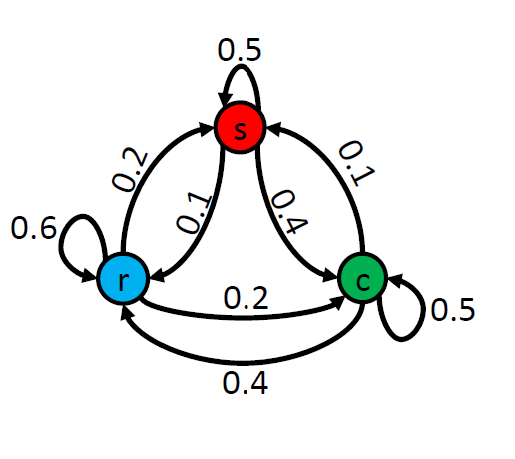
\includegraphics{figures/markov-chain.png}
$$x_{1: T}=s r  c r r c s \quad\quad\quad A= \left[\begin{array}{lll}
0.6 & 0.2 & 0.2 \\
0.1 & 0.5 & 0.4 \\
0.4 & 0.1 & 0.5
\end{array}\right]$$
$$\mathrm{P}\left(X_{1: T}=x_{1: T}\right)=\mathrm{P}\left(X_{1}=s\right) \times 0.1 \times 0.2 \times 0.4 \times 0.6 \times 0.2 \times 0.1$$
\caption{Markov Chain Example}    
\label{fig:markov-chain-example}
\end{figure}

Figure \ref{fig:markov-chain-example} is an example of the Finite State Machine representation of a Markov Chain, which models weather. There are  three states of weather: rainy, sunny, and cloudy. The weather of a given day only depends on the previous day. A sequence of the weather for 7 days is given, which can be thought of as a random walk in the Finite State Machine.  Its probability can be calculated accordingly using the transition matrix and the start probabilities \parencite{miningmassivedatasets}.

\section{Hidden Markov Model}

In the regular Markov chain each state is directly observable. In many applications this is not the case: there can be a non-deterministic process determining the output for each state. We get observations for each time point, but we do not know the state. It is \emph{hidden}. 

We get a two layered probabilistic model. The hidden states are modeled by a regular Markov chain. Then each state has a probabilistic function that generates the observed output. 

\begin{figure}
    \centering
   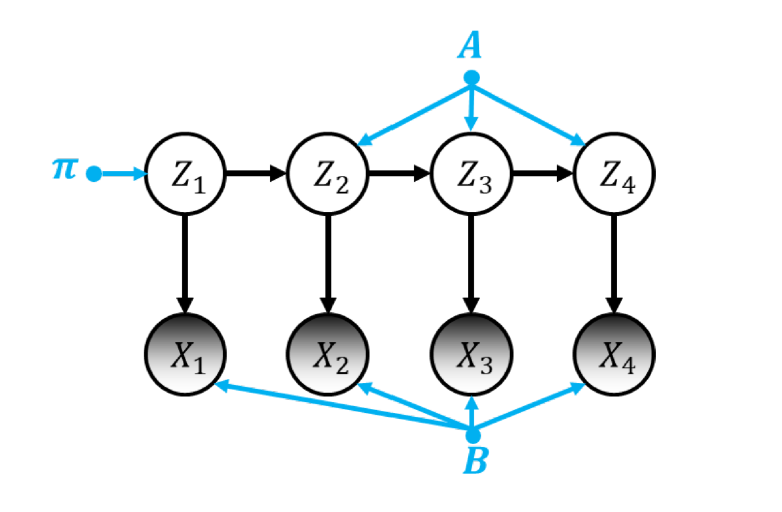
\includegraphics{figures/HMM.png}
\caption{Hidden Markov Model}    
\label{fig:hmm}
\end{figure}

\newpage
To represent this extension of the Markov chain we have to add an additional variable to the parameterization: 

\begin{equation}
\begin{aligned}
&a_{i j}=P\left(s_{t}=j | s_{t-1}=i\right) \quad 1 \leq i, j \leq N \\
&\pi_{i}=P\left(s_{1}=i\right) \quad 1 \leq i \leq N \\
&b_{i}(k)=P\left(X_{t}=o_{k} | s_{t}=i\right) \\
&\sum_{j=1}^{N} a_{i j}=1 ; \quad 1 \leq i \leq N \\
&\sum_{j=1}^{N} \pi_{j}=1 \\
&\sum_{k=1}^{M} b_{i}(k)=1
\end{aligned}
\label{eq:hmm-def}
\end{equation}

The three parameters together are referred to as $\Phi$.

\begin{equation}
\Phi=(\mathbf{A}, \mathbf{B}, \boldsymbol{\pi})
\end{equation}

The parameter $b_{i}(k)$ is called emission probability. It represents the probability of generating output $o_k$ from state $i$. Again, since it is a probability it is constrained: The probabilities of the different outputs of a state have to add up to 1. The specific format of $b$ depends on the chosen probability distribution for the outputs of model. 
The current formulation assumes discrete outputs, which is represented by a categorical distribution and would lead to $b$ being a matrix. One the other hand, when modeling continuous outputs the distribution of choice is the normal distribution. In that case $b$ is a set of means and variances. This paper will focus the continuous case.

On top of the Markov Property Hidden Markov Models have to fulfill a second property: The \emph{output-independence assumption}:

\begin{equation}
P\left(X_{t} |X_{1}, X_{2}, \ldots, X_{t-1}, s_{1}^{t}\right)=P\left(X_{t} | s_{t}\right)
\end{equation}

This property assures that each output only depends on its corresponding state. It is independent of all other outputs \parencite{huang2001spoken}.

How can we use Hidden Markov Models to generate time series? Since HMMs are a generative model it is easy: specify the three parameters $A, B, \pi$ according to the model. Then generate a series of hidden states using the start and transition probabilities. Finally generate the data points according to the emission probabilities. But there is another way: we can learn the parameters from an existing time series. Using those we can then generate a new time-series with similar properties to the training time-series. The learning problem can be solved using the \emph{Forward/Backward algorithm} and the \emph{Baum-Welch algorithm}.

\section{Forward Algorithm}

To learn the parameters $\Phi$ of a Hidden Markov Model to match the characteristics of a given training sequence $X$, we have to be able to assess the likelihood of a sequence for certain parameters. 

\begin{equation}
   P(\mathbf{X} | \Phi)=\sum_{\mathrm{all\:S}} P(\mathbf{S} | \Phi) P(\mathbf{X} | \mathbf{S}, \Phi) 
\end{equation}

The idea is to sum over all possible state sequences $S$ and compute how likely each state sequence is given the parameters and multiply this with the likelihood of these states producing the observed outputs. 

In terms of $A$, $B$, and $\pi$ this becomes:

\begin{equation}
   P(\mathbf{X} | \Phi)=\sum_{\text {all } \mathbf{S}} \pi_{s_{1}} b_{s_{1}}\left(X_{1}\right) a_{s_{1} s_{2}} b_{s_{2}}\left(X_{2}\right) \ldots a_{s_{T-1} s_{T}} b_{s_{T}}\left(X_{T}\right) 
\end{equation}

The underlying issue here is that there are exponentially many, $O(N^{T})$, state sequences to consider. However, there is a more efficient way to compute this that involves storing intermediate results, which saves computation. 

Define forward probability $\alpha$:

\begin{equation}
   \alpha_{t}(i)=P\left(X_{1:t}, s_{t}=i | \Phi\right) 
\end{equation}

The term $X_{1:t}$ represents the observations from time 1 up to time $t$. So $\alpha_{t}(i)$ is the probability that given the parameters $\Phi$ we observe the first $t$ values and are in state $i$ at time $t$.

The convenient thing about $\alpha$ is that it can be recursively defined:

\begin{equation}
\begin{aligned}
&\alpha_{1}(i)=\pi_{i} b_{i}\left(\mathrm{X}_{1}\right) \quad 1 \leq i \leq N \\
&\alpha_{t}(j)=\left[\sum_{i=1}^{N} \alpha_{t-1}(i) a_{i j}\right] b_{j}\left(X_{t}\right) \quad 2 \leq t \leq T ; 1 \leq j \leq N
\end{aligned}
\label{eq:alpha-def}
\end{equation}

Finally, we compute the probability of $X$ by starting at $\alpha_1$ and going up to $\alpha_T$. The probability of the sequence $X$ is:

\begin{equation}
   P(\mathbf{X} | \Phi)=\sum_{i=1}^{N} \alpha_{T}(i) 
  \label{eq:prop-statement}
\end{equation}

By reusing the intermediate values we save computation and the runtime becomes $O(N^2 T)$ \parencite{huang2001spoken}. 

\section{Backwards Algorithm}

Analogous to the Forward Algorithm there is also the Backwards Algorithm. It is defined like this:

\begin{equation}
   \beta_{t}(i)=P\left(X_{t+1:T} | s_{t}=i, \Phi\right) 
\end{equation}

The term $X_{t+1:T}$ refers to the observations from $t+1$ to the end of the sequence. Because of this $\beta$ is evaluated the other way around, giving the algorithm its name. The recursive definition of $\beta$ is this:

\begin{equation}
\begin{aligned}
   &\beta_{T}(i)=0 \quad 1 \leq i \leq N  \\
   &\beta_{t}(i)=\left[\sum_{j=1}^{N} a_{i j} b_{j}\left(X_{t+1}\right) \beta_{t+1}(j)\right] \quad t=T-1 \ldots 1 ; \quad 1 \leq i \leq N
   \label{eq:beta-def}
\end{aligned}
\end{equation}

The base case is the last row of $\beta$. Since there are no observations following this one, it is the probability of the empty set, which is 0 \parencite{huang2001spoken}.

Why we need both the Forward and Backwards algorithm will become clear when looking at the \emph{Baum-Welch algorithm}.

\section{EM Algorithm}

The Baum Welch algorithm is a so called EM-algorithm. Its goal is the same as in Maximum Likelihood Estimation (MLE). We are trying to find parameters that maximize a probability distribution. The difference is that a EM-algorithm also works with incomplete observed data. In the case of Hidden Markov Models this are the hidden states. 

An EM algorithm deals with the issue of missing data in this way: We do MLE using expected instead of actual data. The initial parameters are guessed. Then during each iteration we use the current parameters to compute the expectation of the missing data. With the now complete data we perform MLE to obtain new parameters. This is where the name EM algorithm comes from: E for Expectation and M for Maximization. 
 
Each iteration of the EM algorithm will improve the accuracy of the parameters and they will eventually converge. However, there is no guarantee to find the global maximum this way. We might run into a local maximum. This issue can be avoided by picking good values for the initial guess of parameters. The implementation section will discuss the approach for this.

\section{Parameter Learning - Fully Observed}

In the Baum Welch algorithm the parameters we are trying to estimate are $A$, $B$, and $\pi$. Suppose we have fully observed data for multiple sequences, that is we know both the observations and all the hidden states $X_{1: T_{n}}^{(n)}, s_{1: T_{n}}^{(n)}$. Then we can obtain the parameters using Maximum Likelihood Estimation on this probability distribution:


\begin{equation}
  P(X_{1: T_{n}}^{(n)}, s_{1: T_{n}}^{(n)})=\left(\prod_{k} \pi_{k}^{L(k)}\right)\left(\prod_{i, j} a_{i j}^{N(i, j)}\right)\left(\prod_{i, j} b_{i}(j)^{M(i, j)}\right) 
\end{equation}

Where:

\begin{equation}
  \begin{array}{c}
L(k)=\#\left(s_{1}=k\right) \\
N(i, j)=\#\left(s_{t}=i, s_{t+1}=j\right) \\
M(i, j)=\#\left(s_{t}=i, X_{t}=j\right)
\end{array} 
\end{equation}

It is simpler to obtain the maximum when taking the $\log$:

\begin{equation}
\begin{split}
  \log P=\left(\sum_{k} L(k) \log \left(\pi_{k}\right)\right)+\left(\sum_{i, j} N(i, j) \log \left(a_{i j}\right)\right)  \\
   +\left(\sum_{i, j} M(i, j) \log \left(b_{i}(j)\right)\right) 
\end{split}
\end{equation}

Since each part of the sum only has one parameter in it they can be maximized independently. They all have the form: 

\begin{equation}
   \begin{aligned}
\text{max} \sum_{i} y_{i} \log x_{i} \\
\text{s.t.} \sum_{i} x_{i}=1
   \end{aligned}
  \label{eq:lp-statement}
\end{equation}

The constraint of summing up to one comes from the definition of the HMM parameters in Equation \eqref{eq:hmm-def}. This is a linear programming problem, which can be solved, for example, using Lagrange Multipliers \parencite{huang2001spoken}. The maximum will be achieved when: 

\begin{equation}
  x_{i}=\frac{y_{i}}{\sum_{i} y_{i}} 
  \label{eq:lp-solution}
\end{equation}

Finally, we get these values for the three parameters: 

\begin{equation}
  \hat{a}_{i j}=\frac{N(i, j)}{\sum_{s} N(i, s)} \quad \hat{b}_{i}(j)=\frac{M(i, j)}{\sum_{s} M(i, s)} \quad \hat{\pi}_{k}=\frac{L(k)}{\sum_{s} L(s)} 
\end{equation}

This makes sense intuitively: For $\pi$ the start probability of state $k$ will be the fraction of observed sequences starting in $k$ over total observed sequences. Similarly, the transition probability form state $i$ to state $j$ is the number of observed ``$i$ to $j$'' transitions over total observed transitions \parencite{miningmassivedatasets}. 

\section{Baum-Welch - E-step}

The previous computations assumed we observed the hidden states. This is not the case in the Baum-Welch algorithm and we have to apply the EM approach. For this we reformulate the probability in terms of the expectation of the hidden states $P\left(s_{1: T} | X_{1: T}, \theta_{\text {old}}\right)$, which looks like this:

\begin{equation}
\begin{split}
\mathbb{E}_{P\left(s_{1: T} | X_{1: T}, 
\theta_{\text {old}}\right)}\left[\ln P\left(X_{1: T}, s_{1: T}, \theta_{n e w}\right)\right] 
=\sum_{k} \mathrm{P}\left(s_{1}=k | X_{1: T}, \theta_{\text {old}}\right) \log \left(\pi_{k}^{n e w}\right) \\
+\sum_{i, j} \sum_{t} \mathrm{P}\left(s_{t}=i, s_{t+1}=j | X_{1: T}, \theta_{\text {old}}\right) \log \left(a_{i j}^{n e w}\right) \\
+\sum_{i, j} \sum_{t \in X_t = j} \mathrm{P}\left(s_{t}=i | X_{1: T}, \theta_{o l d}\right)    \log \left(b_{i}(j)^{n e w}\right)
\end{split}
\end{equation}

First we have to compute the expectations: the E-step of the EM-algorithm. Define two intermediate variables $\gamma$ and $\xi$: 

\begin{equation}
  \begin{aligned}
&\mathrm{P}\left(s_{t}=i | X_{1: T}, \theta_{\text {old}}\right) \stackrel{\text { def }}{=} \gamma_{t}(i)\\
&\mathrm{P}\left(s_{t}=i, s_{t+1}=j | X_{1: T}, \theta_{o l d}\right) \stackrel{\mathrm{def}}{=} \xi_{t}(i, j)
\end{aligned} 
\end{equation}

The variable $\gamma_t(i)$ represents the probability to be in state $i$ after $t$ time steps given the observation and old parameters. We already have all the pieces in place to compute this.

From the forward and backward algorithm we get $\alpha_t(i)$ and $\beta_t(i)$, which represent the probability to be in state $i$ at $t$. The condition for $\alpha$ is the observations up to point $t$ and for $\beta$ the observations following point $t$.

\begin{equation}
   \gamma_t(i) = \frac{\alpha_{t}(i) \beta_{t}(i)}{\sum_{s} \alpha_{t}(s) \beta_{t}(s)}
\end{equation}

Multiplying $\alpha$ and $\beta$ together results in the desired probabilities. We then have to normalize to get $\gamma$. 

The variable $\xi$ can also be computed using $\alpha$ and $\beta$. 

\begin{equation}
   \xi_{t}(i, j)=\frac{\mathrm{P}\left(s_{t}=i, s_{t+1}=j, X_{1: T}\right)}{\mathrm{P}\left(X_{1: T}\right)} \propto \mathrm{P}\left(s_{t}=i, s_{t+1}=j, X_{1: T}\right)
\end{equation}

We can break up $X_{1:T}$ like this:

\begin{equation}
   \xi_{t}(i, j) \propto \mathrm{P}\left(s_{t}=i, s_{t+1}=j, X_{1: t}, X_{t+1},X_{t+2:T}\right)
\end{equation}

Now we apply the chain rule three times.

\begin{equation}
  \begin{aligned}
\xi_{t}(i, j) \propto \;  &\mathrm{P}\left(s_{t}=i, X_{1: t}\right) \mathrm{P}\left(s_{t+1}=j | s_{t}=i, X_{1: t}\right) \\
&\mathrm{P}\left(X_{t+2: T} | s_{t}=i, X_{1: t}, s_{t+1}=j\right) \\
&\mathrm{P}\left(\mathrm{X}_{t+1} | s_{t}=i, X_{1: t}, s_{t+1}=j, X_{t+2: T}\right)
\end{aligned} 
\end{equation}

Then we remove unnecessary conditions in the conditional probabilities.

\begin{equation}
\begin{aligned}
\xi_{t}(i, j) \propto \; &\mathrm{P}\left(s_{t}=i, X_{1: t}\right) \mathrm{P}\left(s_{t+1}=j | s_{t}=i\right) \\
&\mathrm{P}\left(X_{t+2: T} | s_{t+1}=j\right) \mathrm{P}\left(\mathrm{X}_{t+1} | s_{t+1}=j\right) \\
\propto \;  & \alpha_{t}(i) a_{i j} \beta_{t+1}(j) b_{j}(x_{t+1})
\end{aligned} 
\end{equation}

At this point we either normalize or compute the original denominator $P(X_{1:T})$ directly using $\alpha$.

\begin{equation}
\begin{aligned}
\xi_{t}(i, j)=&\frac{\alpha_{t}(i) a_{i j} \beta_{t+1}(j) b_{j}(x_{t+1})}{\sum_{u} \sum_{v} \alpha_{t}(u) a_{u v} \beta_{t+1}(v) b_{v}( x_{t+1})} \\
\xi_{t}(i, j)=&\frac{\alpha_{t}(i) a_{i j} \beta_{t+1}(j) b_{j} (x_{t+1})}{\sum_{i=1}^{N} \alpha_{T}(i)}
\label{eq:xi-def}
\end{aligned}
\end{equation}

Having computed $\xi$ and $\gamma$ we have reformulated the probability distribution in terms of expectations, which completes the E-step. We first run the forward and backwards algorithm to obtain $\alpha$ and $\beta$. They each take $O(TK^2)$. Then we compute $\gamma$ and $\xi$, which take $O(TK)$ and $O(TK^2)$ respectively. So the overall runtime of the E-step is $O(TK^2)$ \parencite{miningmassivedatasets}.

\section{Baum-Welch - M-step}

Plugging in the in the expectation values from the E-step in the probability distribution yields this formula for the log likelihood:

\begin{equation}
\begin{aligned}
\mathbb{E}_{P\left(s_{1: T} | X_{1: T}, \theta_{o l d}\right)}\left[\ln P\left(X_{1: T}, s_{1: T}, \theta_{n e w}\right)\right] &=\sum_{k} \gamma_{1}(k) \log \left(\pi_{k}^{n e w}\right) \\
&+\sum_{i, j} \sum_{t} \xi_{t}(i, j) \log \left(a_{i j}^{n e w}\right) \\
&+\sum_{i, j} \sum_{t \in X_t = j} \gamma_{t}(i)   \log \left(b_{i}(j)^{n e w}\right)
\end{aligned}
\end{equation}

In the M-step of the Baum-Welch algorithm we now perform Maximum Likelihood Estimation to compute new values for the parameters $A$, $B$, and $\pi$. Again we have three independent linear programs of the from defined in Equation \eqref{eq:lp-statement}, which can be solved using the solution from Equation \eqref{eq:lp-solution}. 

\begin{equation}
  \pi_{k}^{n e w}=\gamma_{1}(k) 
\end{equation}

By definition the rows of gamma sum up to 1, so a normalizing denominator is not necessary. 

\begin{equation}
   \begin{aligned}
   a_{i j}^{n e w}&=\frac{\sum_{t=1}^{T-1} \xi_{t}(i, j)}{\sum_{i,j}  \sum_{t=1}^{T-1} \xi{t}(i,j)} \\
   &=\frac{\sum_{t=1}^{T-1} \xi_{t}(i, j)}{\sum_{t=1}^{T-1} \gamma_{t}(i)} 
   \end{aligned}
\end{equation}

When summing up $\xi$ the $a_{ij}$ and $b_i(j)$ cancel out because their row are defined to sum up to 1. The denominator can be simplified and expressed using $\gamma$.

\begin{equation}
   b_{i}(j)^{\text {new}}=\frac{\sum_{t \in X_t = j} \gamma_{t}(i) }{\sum_{t=1}^{T} \gamma_{t}(i)}
\end{equation}

When summing over every possible j we consider every time point once, so to normalize we divide by the sum over every time index $t$. Note that this formulation of $b$ only applies for Hidden Markov Models with discrete output. Identifying the subset $t \in X_t=j$ does not make sense in a continuos setting. 

The most complex operation during the M-step is computing $a$, which takes $O(TK^2)$. This makes the overall runtime of one Baum-Welch iteration $O(TK^2)$, where T is the number of training samples and K is the number of hidden states \parencite{miningmassivedatasets}.

\section{Continuos Hidden Markov Model}

While the previous calculations are made under the assumption of discrete outputs, there is only little change required to adapt the Baum-Welch algorithm to the continuos case. There are multiple approaches. One is called semi-continuos and works by assigning a normal distribution with mean $\mu_k$ and variance $\sigma_k$ to each hidden state $k$. This changes the probability distribution in the following way:

\begin{equation}
\begin{aligned}
\mathbb{E}_{P\left(s_{1: T} | X_{1: T}, \theta_{o l d}\right)}\left[\ln P\left(X_{1: T}, s_{1: T}, \theta_{n e w}\right)\right] &=\sum_{k} \gamma_{1}(k) \log \left(\pi_{k}^{n e w}\right) \\
&+\sum_{i, j} \sum_{t} \xi_{t}(i, j) \log \left(a_{i j}^{n e w}\right) \\
&+\sum_{i} \sum_{t} \gamma_{t}(i)    \log \left(\mathcal{N}\left(x_{t} | \mu_{i}, \sigma_{i}^{2}\right)\right.  )
\end{aligned}
\end{equation}

Parameters $\pi$ and $a$ are unchanged, however $b$ is now represented by two variables $\mu$ and $\sigma$. The formula is more complex so the Lagrange Multiplier solution does not work. Thus, we maximize by setting the derivative to 0. 

\begin{equation}
\begin{aligned}
\frac{\partial}{\partial \mu_i} \mathbb{E}[\ln P] &= c \cdot \sum_t \gamma_t(i) (x_t - \mu_i) = 0 \\
\Rightarrow \mu_i &= \frac{\sum_t \gamma_t(i)x_t}{\sum_t \gamma_t(i)}
\end{aligned}
\label{eq:mu-def}
\end{equation}

\begin{equation}
\begin{aligned}
\frac{\partial}{\partial \sigma_i} \mathbb{E}[\ln P] &= \sum_t \gamma_t(i) (\frac{1}{\sigma_i^3}(x_t-\mu_i)^2 - \frac{1}{\sigma_i}) = 0 \\
\Rightarrow \sigma_i^2 &= \frac{\sum_t \gamma_t(i)(x_t - \mu_i)^2}{\sum_t \gamma_t(i)}
\end{aligned}
\label{eq:sigma-def}
\end{equation}

The semi-continuos approach is favorable because it only differs from the discrete approach at this one point during the M-step. It is called semi-continuos because the only available probability distribution is the normal distribution. A more flexible approach is to use Gaussian Mixture Models instead of simple normal distributions, which looks like this: 

\begin{equation}
  b_{j}(\mathbf{x})=\sum_{k=1}^{M} c_{j k} N\left(\mathbf{x}, \boldsymbol{\mu}_{j k}, \boldsymbol{\Sigma}_{j k}\right) 
\end{equation}

A Gaussian Mixture model is a weighted sum of normal distributions. This is powerful since it can approximate any continuos function. For each state there are $M$ different normal distributions each with a mean and variance. Moreover there is $c$, which represents the weights of each distributions for each state. 

The fully continuos approach introduces a lot of complexity including a new parameter $c$, which makes the training computationally expensive. This makes the semi-continuos model a better approach for most applications, including this paper, where the semi-continuos approach is implemented \parencite{huang2001spoken}.
